\chapter{\textbf{Introduction and Background}}
Redundant, accurate flight vehicle localization has been well-documented over several decades~\cite{zhaoCooperativeLocalizationBased2017,rufaSensorFusionUnmanned2014,tennyRobustNavigationUrban2022,kandemirProbabilisticMeasurementMethod2018}. However, as the threat to GPS signals continues to rise, the need for robust pose estimation increases. While robust systems already exist to combat incoming interference, these systems are either proprietary or government controlled, making them infeasible for widespread use. Cheaper, robust systems are critical for the safe future of civilian and military flight vehicles. Commercial aircraft feature a wide sensor suite that works in tandem to provide redundancy and safety critical features to maintain safe flight. These aircraft have the space to install robust sensor suites and the power to run them consistently in all phases of flight (Figure~\ref{fig:weights}), more importantly, the companies that design and build these aircraft also have the budget to afford such expensive sensor suites.

\begin{figure}[!ht]\label{fig:weights}
    \centering
    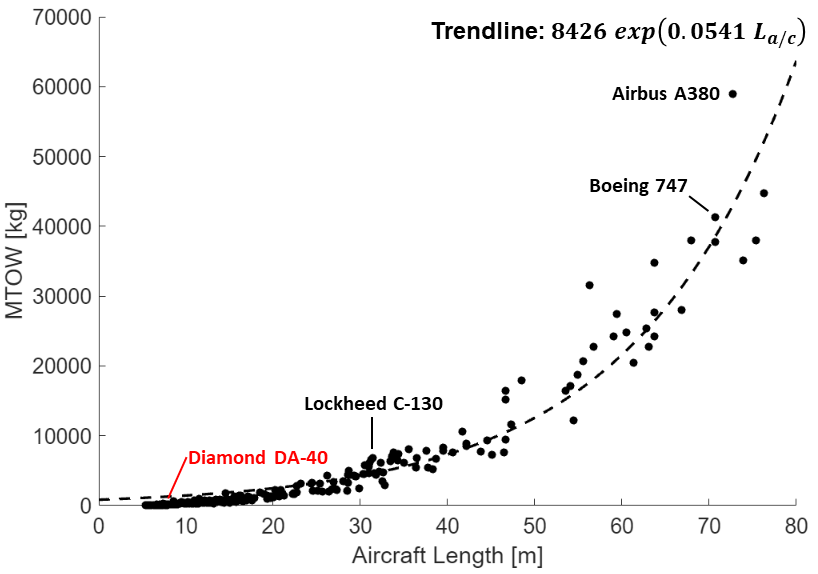
\includegraphics[width=.6\linewidth]{Figures/weights.png}
    \caption{Aircraft with a larger Max Takeoff Operating Weight (MTOW) typically have more space for more complex sensor suites compared to their General Aviation counterparts~\cite{AircraftCharacteristicsDatabase}.}
\end{figure}

Smaller aircraft are not allowed these luxuries, being manufactured with fewer sensors, overall making them less safe. Table~\ref{tbl:sensorsuitecomparison} compares the different sensors onboard a commercial airliner and a civilian general aviation aircraft.

\begin{table}[!ht]\label{tbl:sensorsuitecomparison}
    \caption{Inexhaustive list of sensors available to commercial and general aviation aircraft. (Adapted from~\cite{DiamondAircraftDA401969,customerservicesA380AircraftCharacteristics2020})}
    \centering
    \begin{tabular}{lcc}
        \toprule
        \textbf{Sensor}                    & \textbf{Commercial} & \textbf{General Aviation} \\
        \midrule
        Pitot Tubes                        & \(5\)               & \(2\)                     \\
        Distance Measuring Equipment       & \(2\)               & \(1\)                     \\
        Ultra-High Frequency Sensors       & \(2\)               & \(1\)                     \\
        Very-High Frequency Sensors        & \(3\)               & \(2\)                     \\
        Communication Channels             & \(2\)               & \(2\)                     \\
        Outside Air Temperature Sensors    & \(4\)               & \(1\)                     \\
        Fuel Flow Gauge                    & \(4\)               & \(1\)                     \\
        GPS receivers                      & \(2\)               & \(1\)                     \\
        Inertial Measurement Units         & \(3\)               & \(1\)                     \\
        Satellite Communications           & \(1\)               & {--}                      \\
        Specific Impulse Sensors           & \(6\)               & {--}                      \\
        Weather Radar                      & \(1\)               & {--}                      \\
        Traffic Collision Avoidance System & \(4\)               & {--}                      \\
        Radio Altimeter                    & \(3\)               & {--}                      \\

        \bottomrule
    \end{tabular}
\end{table}

Regardless of components, the sensor suite aboard any flight vehicle is able to provide measurements more often than that of a GPS receiver, so a sensor fusion algorithm is optimal. Because sensor measurements have inherit errors due to a variety of factors, they can wander or drift over time. GPS measurements, although slower, provide measurements that do not drift at the cost of being noisier. Table~\ref{tbl:sensorfusionframeworks} describes the most common sensor fusion frameworks for GPS and INS platforms. More details on each these frameworks can be found in Chapter 4.
\begin{table}[!ht]\label{tbl:sensorfusionframeworks}
    \caption{Common sensor fusion frameworks used for GPS and INS collection platforms}
    \centering
    \begin{tabular}{cll}
        \toprule
        \textbf{Name}            & \textbf{Level of Measurement}      & \textbf{Advantages}              \\
        \midrule
        \textit{Loosely-Coupled} & Position and Velocity              & Simplicity, Redundancy           \\
        \textit{Tightly-Coupled} & Pseudorange and Doppler            & Observability, Robustness        \\
        \textit{Deeply-Coupled}  & Inphase and Quadrature Correlators & Robustness, Optimal Architecture \\
        \bottomrule
    \end{tabular}
\end{table}

This work presents a deeply-coupled sensor fusion algorithm tied into a Vector Tracking (VT) Software Defined Receiver (SDR). Of the three types of GPS and INS sensor fusion frameworks, it is well-documented that deep-coupling provides higher resistance to signal interference and can operate with less than four satellites for a limited time~\cite{wattsGPSGLONASSL12019}. The benefits of the closed-loop navigation framework (vector tracking) enables a coupling of measurements between satellites; this provides stronger tracking performance in GPS-challenged environments where the signal to noise ratio is lower due to interference~\cite{grierPositionNavigationTiming}.

The proposed navigation filter is not considered a full-replacement of existing sensor coupling solutions, but instead can be utilized as a short-term, reliable source of pose and attitude estimation in scenarios of GPS degradation, or when the aforementioned sensors are providing faulty measurements.

\section{\textbf{Prior Art}}
The objective of this thesis is to investigate the efficacy of flight vehicle state estimation in GPS-degraded conditions by utilizing a deeply-coupled FVDM\@. This thesis will analyze the performance through use of a deeply-coupled sensor fusion algorithm utilizing the state propagation of a FVDM and GPS correlator measurements. The idea of fusing a dynamic model and GPS measurements together on a flight vehicle is a recent development, tied with increased computer performance. The following subsections highlight the work performed by other authors and their contributions to the field.
\subsection{\textbf{Sensor Fusion Overview and Variation}}
Sensor fusion between GPS and other sensors aboard flight vehicles has existed for years and continues to be developed. A precise, accurate, and robust navigation solution is achievable when redundant, expensive, and high-quality sensor are installed. More information about the sensors found aboard commercial aircraft and smaller aircraft can be found in~\cite{airbuscustomerservicesAirbusA380Aircraft2020} and~\cite{DiamondAircraftDA401969}, respectively. Salmon~\cite{salmonExperimentalExplorationLowCost2015} provides an exploratory analysis using ground vehicles and their sensors complimented with a Ground Vehicle Dynamic Model (GVDM) in a tightly-coupled GPS/INS/GVDM sensor fusion framework. The work of Rhudy~\cite{rhudyDynamicModelaidedSensor2017} is similar to the research presented in this thesis as they present use of known controller inputs into a propriety nonlinear flight vehicle model to perform GPS sensor fusion with low-cost IMUs. The following section explores the work of previous authors and the advances of sensor fusion between GNSS measurements and vehicle dynamic models.

\subsection{\textbf{Vehicle Dynamic Model Sensor Fusion}}
One of the more common ways to simulate and model a flight vehicle is to use known aerodynamic coefficients tied in with classical flight dynamics to propagate the states in time. The NAVION aircraft model is a nonlinear mathematical aircraft model that uses known aerodynamic coefficients from a single propeller fixed wing Navion aircraft~\cite{nelsonFlightStabilityAutomatic1998}. Rhudy~\cite{rhudyDynamicModelaidedSensor2017} uses the NAVION model included in a loosely-coupled sensor fusion framework with IMU and GPS measurements.~\cite{rhudyDynamicModelaidedSensor2017} focuses on using a known aircraft model with incoming piloted control inputs to predict the attitude of the aircraft in time. Khaghani and Skaloud~\cite{khaghaniAutonomousVehicleDynamic2016} simulate a UAV using initially, known aerodynamic coefficients but feature the coefficients in their loosely-coupled framework to continuously estimate these variables in their vehicle model. Online estimation of the aerodynamic coefficients allows the model to generalizable, further allowing it to be used on a wide array of aircraft with a similar configuration. Both papers fuse the dynamic model with GPS and IMU measurements at the position and velocity level (loosely-coupled).~\cite{rhudyDynamicModelaidedSensor2017} uses an Unscented Kalman Filter (UKF) in the navigation filter for \"ease of implementation\" while Khaghani~\cite{khaghaniAutonomousVehicleDynamic2016,khaghaniAssessmentVDMbasedAutonomous2018} uses a 47-state Extended Kalman Filter (EKF). Both Rhudy and Khaghani use simulation environments to perform a Monte-Carlo analysis. Each IMU is modeled with a constant bias and integrated white noise as a first-order Gauss-Markov process with numbers that mirror a MEMs quality IMU\@. Both~\cite{khaghaniAutonomousVehicleDynamic2016} and~\cite{rhudyDynamicModelaidedSensor2017} models GPS measurements as white noise with a variance of 1 meter in the North, East, and Down directions. Three years later, Khaghani and Skaloud~\cite{khaghaniAssessmentVDMbasedAutonomous2018} improve the original filter implementation by adding a barometer sensor to the measurement update along with the already standing IMU and GPS measurements. From their 2016 publication, the Monte-Carlo analysis showed unbounded error growth once the GPS outage started, leading to growing errors in aerodynamic coefficient estimates. The additional measurements provided by the barometer aid the overall position solution by providing observability in the altitude estimates. In 2020,~\cite{mwenegohaModelbasedTightlyCoupled2020} innovated upon the 2016 work of Khaghani by coupling the FVDM, IMU, and GPS measurements within a tightly coupled navigation filter. The focus of this work was the performance of the state estimates in scenarios where the receiver had sparse satellite visibility of two and three satellites for a short period.~\cite{mwenegohaModelbasedTightlyCoupled2020} further proved the efficacy of utilizing a FVDM within a sensor fusion framework by conduction live-sky experiments via a modified remote controlled aircraft.

\subsection{\textbf{Other Types of Flight Vehicle Sensor Fusion}}
Other research to localize flight vehicles in GPS-degraded environments revolves around fusing together multiple sensors including Ultra Wide Band (UWB) radios, LiDAR and vision-based algorithms. Dong~\cite{dongIntegratedUWBIMUVisionFramework2022} integrates IMU, UWB, and computer vision for the autonomous approach and landing of a small UAV onto a moving platform. The vision framework operates on identifying and tracking independent ArUco markers to calculate the size of the landing zone. The IMU and UWBs work in tandem in estimating the states of the UAV and distance to the landing platform. The UWB radio provide updates at a high frequency but suffer from noise and dropouts when the UAV is farther away from the landing platform~\cite{dongIntegratedUWBIMUVisionFramework2022}. Gr\'of~\cite{grofPositioningAircraftRelative2022} develops a similar algorithm for detecting a runway using a down-view monocular camera, barometer readings, IMU, and previously recorded air data. Because of the camera, both of the aforementioned papers provide bounded results for pose and attitude estimation. Also because of the camera, the system is more complex and expensive, two things avoided in this work.

\section{\textbf{Field Contributions}}
The focus of the research presented in this thesis is the development of a deeply-integrated FVDM with GPS L1 C/A correlator-level measurements. An evaluation of pose and attitude estimation performance of the proposed navigation filter in GPS-degraded and GPS denied environments is also studied. Taking that into consideration, the following contributions to the field are made:
\begin{itemize}
    \item Determination of the optimal flight vehicle model to use in the navigation algorithm when considering complexity and computational performance.
    \item Comparative analysis of multiple flight scenarios reflecting realistic flight plans and GPS degradation.
    \item Analysis of deeply-coupled sensor fusion algorithm using the flight vehicle model and simulated GPS measurements to determine the efficacy of safe localization.
\end{itemize}

\section{\textbf{Thesis Outline}}
The rest of this work follows a description of the physical systems modeled in the FVDM, description of a scalar tracking SDR, presentation of the VT algorithms, and the proposed navigation filter framework. After a presentation of the methodology, performance analyses of the navigation filter using Monte-Carlo simulations are shown. Wrapping up, final conclusions about the investigation are made and future work considerations are presented.